\chapter{Release 2}
\addcontentsline{toc}{chapter}{Release 2}
\markboth{Release 2}{Release 2}
\renewcommand\fbox{\fcolorbox{blue}{white}}
\label{chap:release2}
% section starts from 1 
%\minitoc

\section*{Introduction}

Ce chapitre présente la deuxieme version de notre application.Il est composé de quatre sprints qui ont été réalisés en 8 semaines. Nous avons commencé par l'ajout de la fonctionnalité d'authentification a l'aide en utilisant l'OIDC, puis nous avons ajouté la fonctionnalité de gestion de profile, absence et de delegation. Enfin, nous avons ajouté la fonctionnalité de consultation des statistiques. Dans ce chapitre, nous décrirons en détail les fonctionnalités de chaque sprint, les défis que nous avons rencontrés et les solutions que nous avons apportées pour les surmonter.

Release 2 : (Du 3 Avril au 27 Mai 2023)

\fbox{\begin{minipage}{30em}
  \textbf{Organisation des sprints :} \\
  Cette release contient les quatre sprints:
  \begin{itemize}
    \item \textbf{Sprint 7:} Gestion d'authentification OIDC et verification biometrique.
    \item \textbf{Sprint 6:} Gestion du Profile, d'absence et de délégué.
    \item \textbf{Sprint 7:} Consultation des statistique
    \item \textbf{Sprint 8:} .....
  \end{itemize}
\end{minipage}}

\section{Sprint 7 (Consultation des statistique)}

\subsection{Sprint Goal}
L'objectif de ce sprint est de permettre à l'utilisateur de consulter les statistiques de ses documents et consulter les documents a l'aide de filtre rapide de statistique.

\subsection{Sprint Backlog}


\begin{adjustwidth}{-1cm}{}
  % \usepackage{longtable}
    
    \begin{longtable}{|c|p{6cm}|c|p{6cm}|c|}
      % \centering
      \hline
      \textbf{ID} & \textbf{User story} & \textbf{ID}  & \textbf{Tâche} & \textbf{Durée} \\
      \hline
      \multirow{2}{*}{1} & En tant qu'utilisateur, je veux pouvoir visualiser les statistiques de l'application afin de suivre l'évolution de l'application.
      & 1.1 & Préparer les interfaces sur Figma. & \multirow{3}{*}{2.5 Jour} \\
      \cline{3-4}
      & & 1.2 & Développer le composant de statistique a une valeur. & \\
      \cline{3-4}
      & & 1.3 & Développer le composant de statistique a plusieurs valeurs. & \\
      \cline{3-4}
      & & 1.4 & Développer la fonction qui recuperer et ranger les statistiques. & \\
      & & 1.5 & Développer la fonction qui permet de visualiser les statistiques. & \\
      % & & 1.6 & Développer la fonction qui permet de filtrer les documents par statistique. & \\
      \cline{1-5}
      \multirow{2}{*}{2} & En tant qu'utilisateur, je veux pouvoir consulter les documents a l'aide de filtre rapide afin de trouver les documents que je cherche. & 2.1.& Ajouter la fonction de filtre a l'interface de consultation des statistiques. & \multirow{2}{*}{0.5 Jour} \\
      \cline{3-4}
      & & 2.2 & Développer la fonction qui permet de filtrer les documents par statistique. & \\
      \cline{1-5}
      \multirow{2}{*}{3} & En tant qu'utilisateur, je veux pouvoir refraichir les données de l'application afin de voir les dernières informations. & 3.1.& Ajouter l'interface de rafraichissement des données a chaque page possible. & \multirow{2}{*}{0.5 Jour} \\
      \cline{3-4}
      & & 3.2 & Développer la fonction qui permet de rafraichir les données de chaque page. & \\
      \cline{1-5}
  \hline
  \caption{Sprint backlog du Sprint 7}
  \label{tab:sprint-backlog-7}
\end{longtable}
\end{adjustwidth}


\subsection{Implémentation du Sprint 7}
\textbf{•	Diagramme de cas d'utilisation du sprint 7}

% add image
\begin{figure}[H]
  \centering
  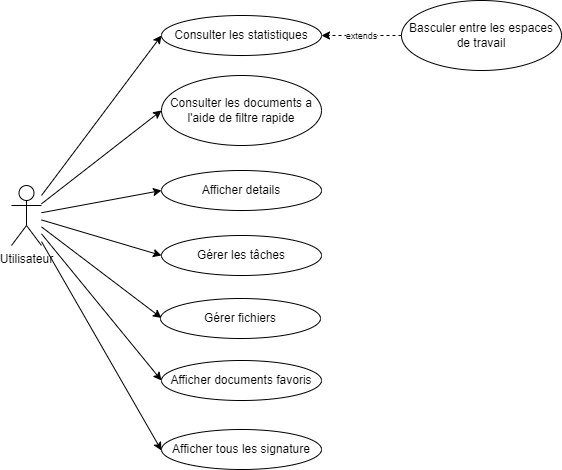
\includegraphics[width=0.4\textwidth]{use_case_sprint_7}
  \caption{Diagramme de cas d'utilisation du sprint 7}
  \label{fig:UseCaseDiagramSp71}
\end{figure}

\subsubsection{Analyse des besoins:}
\textbf{•	Description textuelle de cas d'utilisation « Consulter les statistiques »}

\begin{longtable}{|p{5cm}|p{10cm}|}
\hline
\textbf{Cas d'utilisation}&Consulter les statistiques\\
\hline
\textbf{Acteurs}&Utilisateur\\
\hline
\textbf{Pré Condition}&L'utilisateur est authentifié\\
\hline
\textbf{Post Condition}&Consultation des statistiques\\
\hline
\textbf{Scénario Nominal}&
\vspace{-\baselineskip}
\begin{enumerate}
  \setcounter{enumi}{1}
      \item [2.1] L'utilisateur clique sur le bouton « Accueil »
      \item [2.2] Le système affiche les statistiques
\end{enumerate}\\
\hline
\textbf{Scénario d'exception}&Erreur de connexion\\
\hline
\caption{Description textuelle du diagramme de cas d'utilisation « Consulter les statistiques »}
\label{tab:use_case_consulter_statistiques}
\end{longtable}

\textbf{•	Description textuelle de cas d'utilisation « Consulter les documents a l'aide de filtre rapide »}

\begin{longtable}{|p{5cm}|p{10cm}|}
\hline
\textbf{Cas d'utilisation}&Consulter les documents a l'aide de filtre rapide\\
\hline
\textbf{Acteurs}&Utilisateur \\
\hline
\textbf{Pré Condition}&L'utilisateur doit être authentifié\\
\hline
\textbf{Post Condition}&Consultation des documents a l'aide de filtre rapide\\
\hline
\textbf{Scénario Nominal}&
\vspace{-\baselineskip}
\begin{enumerate}
    \setcounter{enumi}{1}
      \item L'utilisateur clique sur l'une des widget
      \item Le système affiche les documents correspondant au filtre
\end{enumerate}\\
\hline
\textbf{Scénario d'exception}&Erreur de connexion\\
\hline
\caption{Description textuelle du diagramme de cas d'utilisation « Consulter les documents a l'aide de filtre rapide »}
\label{tab:use_case_consulter_documents_filtre_rapide}
\end{longtable}

\textbf{•	Description textuelle de cas d'utilisation « Refraichissement
des données »}

% Note:
\textbf{Note: Cette fonctionnalité est disponible sur la page d'accueil, la page de consultation des documents favoris, la page de consultation d'un document et la page des signatures, mais pour des raisons de lisibilité, nous avons choisi de ne pas répéter la description textuelle de ce cas d'utilisation.}

\begin{longtable}{|p{5cm}|p{10cm}|}
\hline
\textbf{Cas d'utilisation}&Refraichissement des données\\
\hline
\textbf{Acteurs}&Utilisateur \\
\hline
\textbf{Pré Condition}&L'utilisateur doit être authentifié\\
\hline
\textbf{Post Condition}&Refraichissement des données\\
\hline
\textbf{Scénario Nominal}&
\vspace{-\baselineskip}
\begin{enumerate}
    \setcounter{enumi}{1}
      \item L'utilisateur glisse son doigt vers le bas sur l'écran
      \item Le système affiche les dernières données
\end{enumerate}\\
\hline
\textbf{Scénario d'exception}&Erreur de connexion\\
\hline
\caption{Description textuelle du diagramme de cas d'utilisation « Refraichissement des données »}
\label{tab:use_case_refraichissement_donnees}
\end{longtable}

\begin{figure}[H]
  \centering
  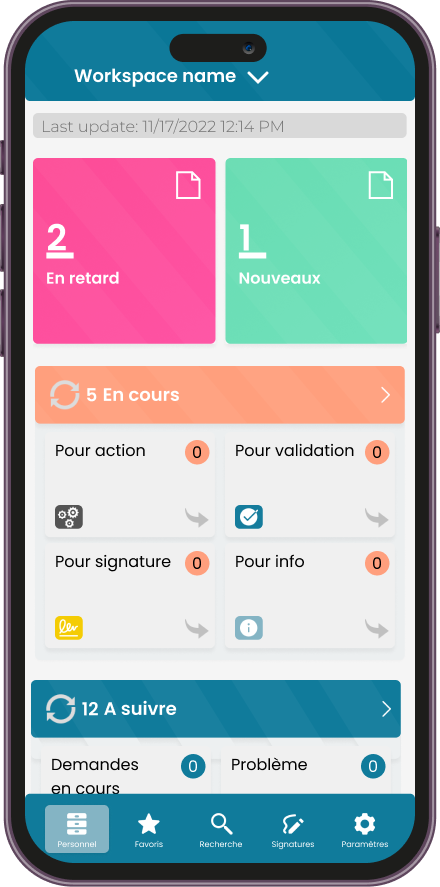
\includegraphics[width=0.35\textwidth]{design_statistique}
  \caption{Maquette de la page de statistique}
  \label{fig:design_statistique}
\end{figure}


Pour avoir une représentation temporelle des interactions entre les objets de notre système et de la chronologie des messages échangés entre eux et avec les acteurs nous avons réalisé les diagrammes de séquence représentés ci-dessous

\begin{figure}[H]
  \centering
  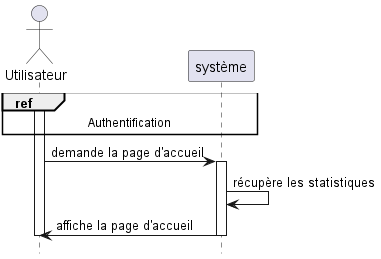
\includegraphics[width=0.7\textwidth]{out/diagrams/sprint7/view_stats/view_stats}
  \caption{Diagramme de séquence de cas d'utilisation « Consulter les statistiques »}
  \label{fig:sequence_view_stats}
\end{figure}

\begin{figure}[H]
  \centering
  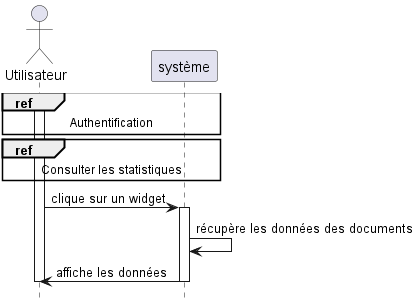
\includegraphics[width=0.7\textwidth]{out/diagrams/sprint7/docs_quick_filter/docs_quick_filter}
  \caption{Diagramme de séquence de cas d'utilisation « Consulter les documents a l'aide de filtre rapide »}
  \label{fig:sequence_docs_quick_filter}
\end{figure}

\textbf{Note: Cette fonctionnalité est disponible sur la page d'accueil, la page de consultation des documents favoris, la page de consultation d'un document et la page des signatures, mais pour des raisons de lisibilité, nous avons choisi de ne pas répéter le diagramme de séquence de ce cas d'utilisation.}
\begin{figure}[H]
  \centering
  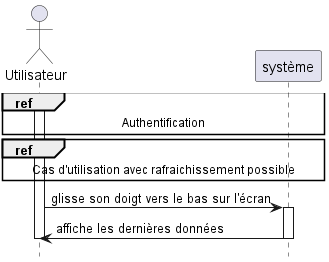
\includegraphics[width=0.7\textwidth]{out/diagrams/sprint7/refresh_data/refresh_data}
  \caption{Diagramme de séquence de cas d'utilisation « Refraichissement des données »}
  \label{fig:sequence_refresh_data}
\end{figure}


\subsubsection{Analyse détaillée}
La présentation de démarche d'analyse fonctionnelle d'un sprint est très importante pour la satisfaction d'un client parce qu'elle consiste à caractériser les fonctions offertes par un produit.
Donc, nous allons faire l'analyse des différents cas d'utilisation en utilisant le diagramme de classes d'analyse.


% spacing between paragraphs
\setlength{\parskip}{1em}
% spacing left
\setlength{\parindent}{0em}

\textbf{•	Diagramme de classe d'analyse de sprint 7 }


\begin{figure}[H]
  \centering
  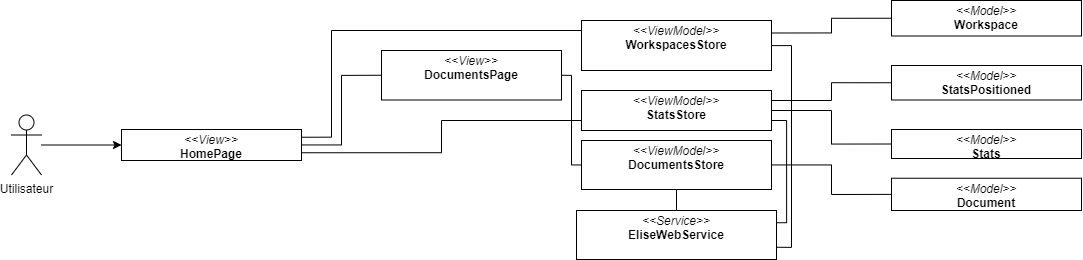
\includegraphics[width=1\textwidth]{dca_sprint7}
  \caption{Diagramme de classe d'analyse de sprint 7}
  \label{fig:class_analyse_sprint7}
\end{figure}


\subsubsection{Conception}

Après la présentation des diagrammes d'analyse, nous avons présenté dans cette partie les diagrammes de conception.\\ 
Nous allons présenter dans cette partie les diagrammes de conception de sprint 7. \\
\textbf{•	Diagramme de classe de conception de sprint 7}

% add image
\begin{figure}[H]
  \centering
  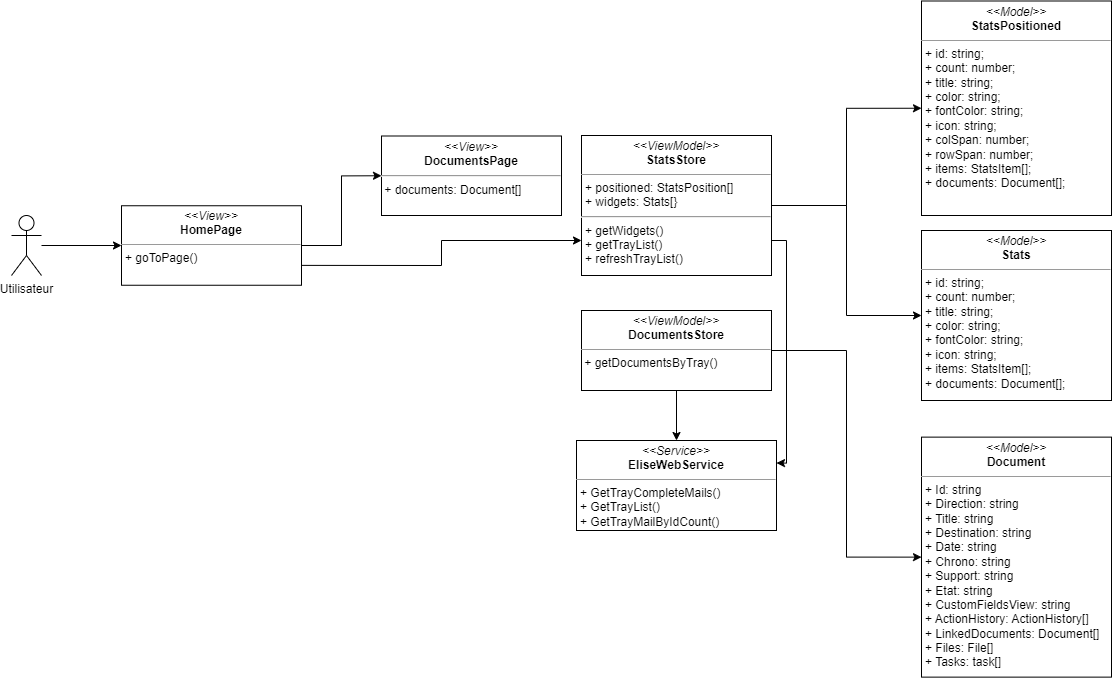
\includegraphics[width=1\textwidth]{dcc_sprint7}
  \caption{Diagramme de classe de conception de sprint 7}
  \label{fig:class_diagram_5}
\end{figure}


\begin{figure}[H]
  \centering
  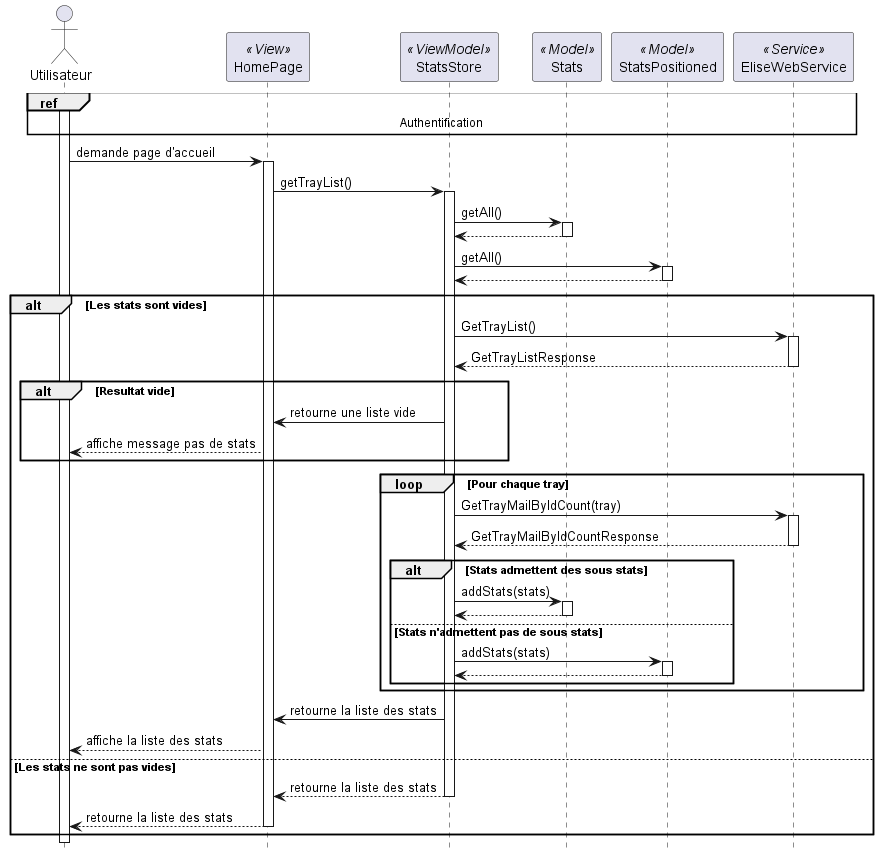
\includegraphics[width=1\textwidth]{out/diagrams/sprint7/sequence_view_stats/sequence_view_stats}
  \caption{Diagramme de séquence de conception de cas d'utilisation « S'Consulter les statistiques »}
  \label{fig:sequence_conception_consulter_statistiques}
\end{figure}

\textbf{Note: Cette fonctionnalité est disponible sur la page d'accueil, la page de consultation des documents favoris, la page de consultation d'un document et la page des signatures, mais pour des raisons de lisibilité, nous avons choisi de ne pas répéter le diagramme de séquence de ce cas d'utilisation.}

\begin{figure}[H]
  \centering
  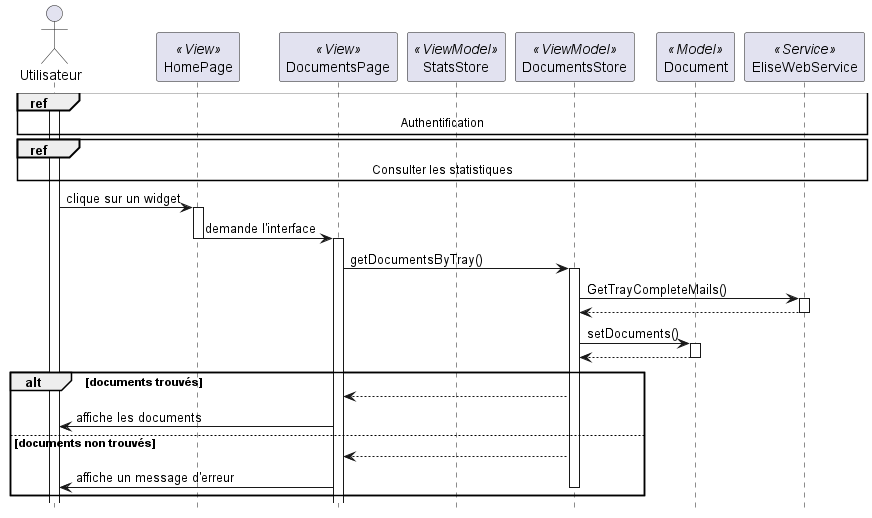
\includegraphics[width=1\textwidth]{out/diagrams/sprint7/sequence_docs_quick_filter/sequence_docs_quick_filter}
  \caption{Diagramme de séquence de conception de cas d'utilisation « Consulter les documents a l'aide de filtre rapide »}
  \label{fig:sequence_conception_consulter_documents_filtre_rapide}
\end{figure}

\begin{figure}[H]
  \centering
  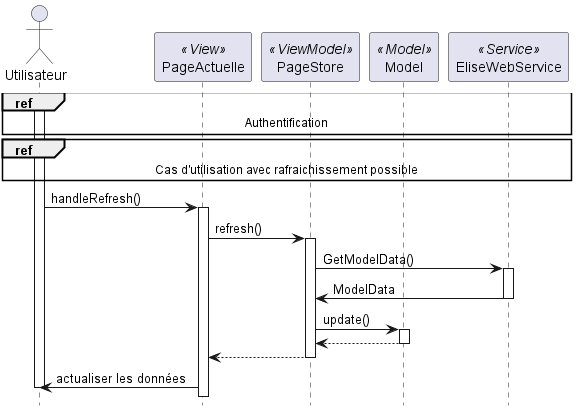
\includegraphics[width=1\textwidth]{out/diagrams/sprint7/sequence_refresh_data/sequence_refresh_data}
  \caption{Diagramme de séquence de conception de cas d'utilisation « Refraichissement des données »}
  \label{fig:sequence_conception_refraichissement_donnees}
\end{figure}

\subsubsection{Réalisation}

Après la présentation des diagrammes d'analyse, nous avons présenté dans cette partie des captures d'écran de l'application.

% add image
\begin{figure}[H]
  \centering
  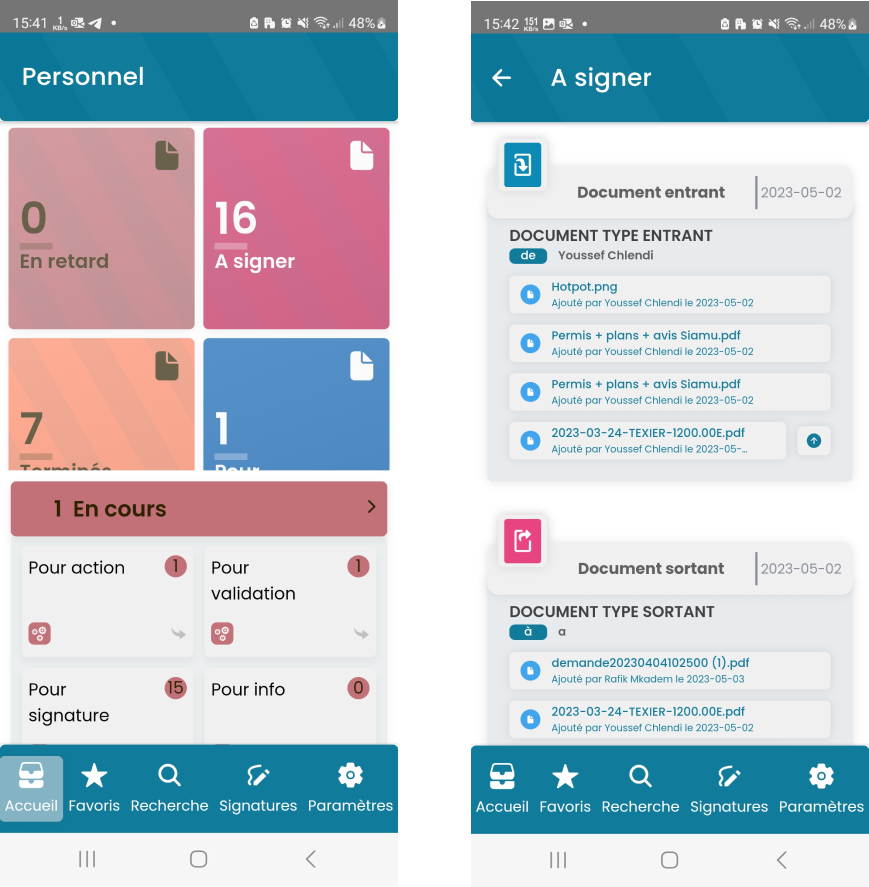
\includegraphics[width=0.7\textwidth, height=0.7\textheight,keepaspectratio=true]{realisation_sprint7}
  \caption{Les interfaces de consultation des statistiques et des documents à l'aide de filtre rapide}
  \label{fig:realisation_sprint7}
\end{figure}

\subsection{Sprint Review}
Suite à cette Technical Story, nous avons pu réaliser les fonctionnalités suivantes :
\begin{itemize}
  \item \textbf{Consulter les statistiques :} Cette fonctionnalité permet à l'utilisateur de consulter les statistiques des documents et des signatures.
  \item \textbf{Consulter les documents à l'aide de filtre rapide :} Cette fonctionnalité permet à l'utilisateur de consulter les documents à l'aide de filtre rapide.
  \item \textbf{Rafraichissement des données :} Cette fonctionnalité permet à l'utilisateur de rafraichir les données.
\end{itemize}

\subsection{Sprint Retrospective}

\begin{itemize}
  \item \textbf{Ce qui a bien fonctionné :}
  \begin{itemize}
    \item Nous avons pu réaliser toutes les fonctionnalités prévues pour ce sprint.
  \end{itemize}

    \item \textbf{Ce qui n'a pas bien fonctionné :}
    \begin{itemize}
      \item Nous avons eu des difficultés à réaliser la fonctionnalité de consultation des statistiques.
    \end{itemize}
      
\end{itemize}
